% 由题面坐标重建，左图取 t=1/4，右图取 t=3/4，使用相同横纵比例。
% K=(0,2+2t^2) 是 QR 与 y 轴交点，L=(0,t+1/t) 是 PQ 与 y 轴交点。
\begin{center}
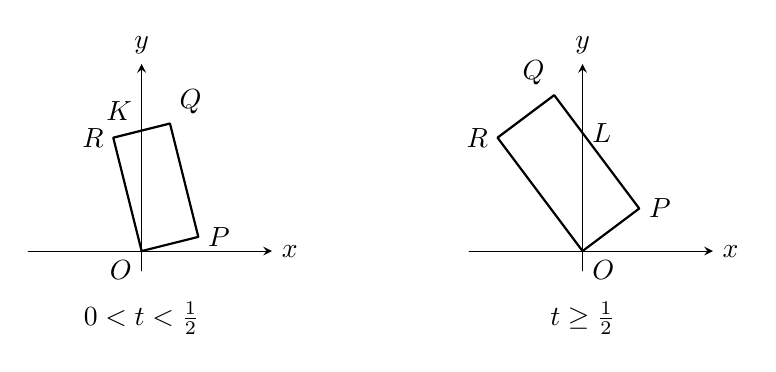
\begin{tikzpicture}[x=0.72cm,y=0.72cm,>=stealth,line cap=round,line join=round]
  \begin{scope}
    \draw[->] (-2,0)--(2.3,0) node[right] {$x$};
    \draw[->] (0,-0.35)--(0,3.3) node[above] {$y$};
    \coordinate (Oa) at (0,0);
    \coordinate (Pa) at (1,0.25);
    \coordinate (Qa) at (0.5,2.25);
    \coordinate (Ra) at (-0.5,2);
    \coordinate (Ka) at (0,2.125);
    \draw[thick] (Oa)--(Pa)--(Qa)--(Ra)--cycle;
    \node[below left] at (Oa) {$O$};
    \node[right] at (Pa) {$P$};
    \node[above right] at (Qa) {$Q$};
    \node[left] at (Ra) {$R$};
    \node[above left] at (Ka) {$K$};
    \node[below] at (0,-0.72) {$0<t<\frac12$};
  \end{scope}
  \begin{scope}[xshift=5.6cm]
    \draw[->] (-2,0)--(2.3,0) node[right] {$x$};
    \draw[->] (0,-0.35)--(0,3.3) node[above] {$y$};
    \coordinate (Ob) at (0,0);
    \coordinate (Pb) at (1,0.75);
    \coordinate (Qb) at (-0.5,2.75);
    \coordinate (Rb) at (-1.5,2);
    \coordinate (Lb) at (0,2.083333333333);
    \draw[thick] (Ob)--(Pb)--(Qb)--(Rb)--cycle;
    \node[below right] at (Ob) {$O$};
    \node[right] at (Pb) {$P$};
    \node[above left] at (Qb) {$Q$};
    \node[left] at (Rb) {$R$};
    \node[right] at (Lb) {$L$};
    \node[below] at (0,-0.72) {$t\ge\frac12$};
  \end{scope}
\end{tikzpicture}
\end{center}
